\documentclass[12pt,a4paper]{article}
\usepackage{geometry}
\usepackage[numbers]{natbib}
\usepackage{amssymb, amsmath}
\usepackage{graphicx}
\usepackage{grffile}
\graphicspath{{../Figures/}}
\usepackage{gensymb}
\usepackage[font=small]{caption}
\usepackage[utf8]{inputenc}
\usepackage[english]{babel}
\usepackage{fancyhdr}
\usepackage[raggedright]{titlesec}
\usepackage{subcaption}
\usepackage{multirow}
\usepackage{dirtytalk}
\usepackage{framed}
\usepackage[normalem]{ulem}
\usepackage[pdftex,breaklinks]{hyperref}
\hypersetup{
  colorlinks   = true, %Colours links instead of ugly boxes
  urlcolor     = green, %Colour for external hyperlinks
  linkcolor    = blue, %Colour of internal links
  citecolor   = red %Colour of citations
}


\begin{document}
\author{Katrina Ashton}


\pagestyle{fancy}
\fancyhf{}
\rhead{\thepage}
\lhead{u5586882}

\section{What I've done}
\begin{itemize}
\item Got data to test new RealSense for Vicon interference (haven't checked yet, by eye there are more points with no data but it's otherwise ok)
\item Got some data from my quadcopter (circle trajectory).
\item Wrote background section of report.
\item Working on re-installing ubunutu on my laptop and getting ROS working. Ended up only getting it installed on a virtual machine.
\item Working on extracting image data from ROS bag so that it can be used with my existing code. Although I will probably eventually want to write code to run on the ros data directly.
%\item{Added more to the appendices for the final report draft}
\end{itemize}

\section{Parts of report to look at}
\begin{itemize}
\item Background (section 4, page 4)
\end{itemize}

\section{Questions}
\begin{itemize}
\item What do you want me to cover in the lit review? I think right now I just have a section on ICP, which we might not even be using anymore. I'll probably need a general section on registration techniques and possibly some more specialised ones (might have to be in second draft). But I'm not sure if there's anything else you think I need.
\end{itemize}

\section{Comments}
\begin{itemize}
\item Still having issues with the SD card on the quad. If I connect it up to the monitor first and run chmod 777 from there it works fine via SSH. But if I try to run chmod 777 from SSH it doesn't work. Not really sure how to fix it, but I can work around it. 
\item Collecting the data took a really long time due to various issues with the quad and the afore-mentioned SD card issues. So I'm running a bit behind schedule on other aspects. 
\item I got some data but the quad was flying too low. I did another run with it higher, but I think something stuffed up with the SD card/reindexing because the rosbag doesn't have the data. (I only got around to actually trying to process the data on Thursday night because it took me so long to get it). There might be another copy on the TX2 (although I think for this one I recorded directly to the SD card, so probably not) or I might have to fly again after our meeting.
\item I worked out how to fix that a problem I was running into while trying to install ROS last time. So I had another go of installing ROS on my dual boot, but it won't let me do it. I think some of the previous attempts kind of half-completed and are now stopping it from trying to install. I did a bit of googling and tried to fix it but couldn't get it working.
\item I tried to reinstall ubuntu on my dual boot, but I couldn't get it working (I downloaded a new image and set up a bootable USB but it kept freezing partway through when I tried to install or try ubuntu. I might try again later with a different USB and/or powered USB hub -- I remember my USB slots had a few issues after I tried running the old RealSense through them so that migth be part of the issues). I set up a virtual machine running ubuntu (I had to use the iso directly instead of from the USB). That should be ok for playing rosbags but I'm not sure if I can use it for flying the quad.
\item Kabsch seems to work ok for the quad data now that there is actually a translation, however it seems like far away points don't quite match up (although note that I'm not using the right scaling factor). I haven't implemented RANSAC properly for Kabsch yet though.
\item I haven't done the ground truth yet, but the trajectory should be circle of radius approximately 1.2m with the the camera facing inwards.
\item Not sure if it's a problem with the recording or with extracting the images from the rosbag, but I have many more depth images than rgb images (around 500 vs around 50), and some of the rgb images are very close while some are far apart. For now I just deleted the close ones.
\item I'm fairly busy week 6 (midsem, other assignments, social engagement) so I've scheduled less work for then. I should be able to get a fair bit done over the break though as I don't think my other courses are planning to give out very big assignments over the break.
\end{itemize}

\begin{figure}[h]
  \centering
  \includegraphics[width=60mm]{../data/quad1/rgb/1533792214.08.png}
  \caption{Example RGB image, top of boxes is cut off}
  \label{f: quad low rgb}
\end{figure}

\begin{figure}[h]
  \centering
  \begin{subfigure}[t]{0.5\textwidth}
  \centering
  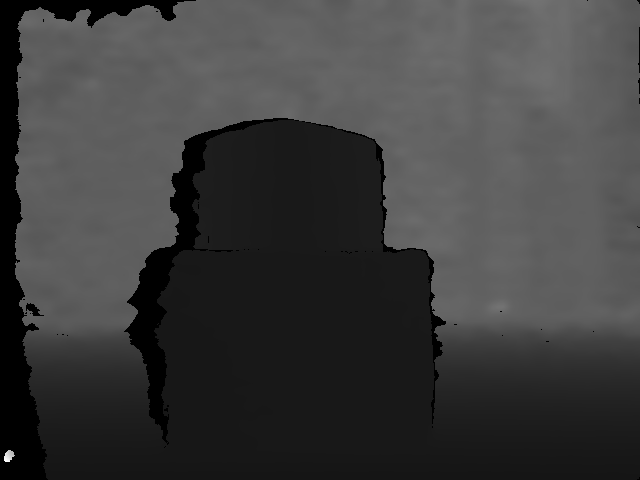
\includegraphics[width=60mm]{21-no-vicon/depth/0.001719236.png}
  \caption{Depth image with no Vicon}
  \end{subfigure}%
  ~
  \begin{subfigure}[t]{0.5\textwidth}
  \centering
  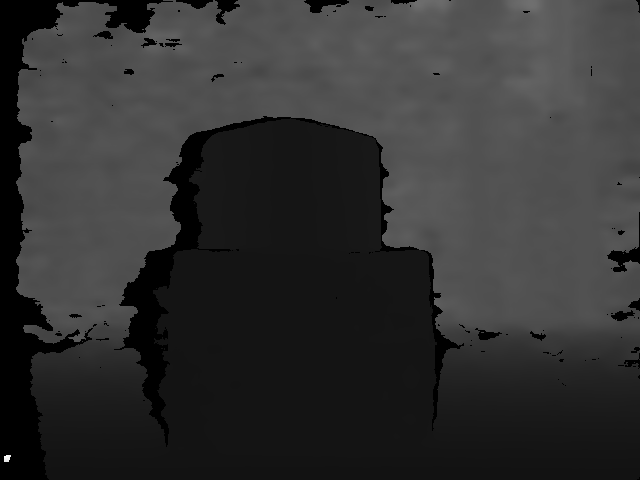
\includegraphics[width=60mm]{25-vicon/depth/0.001719236.png}
  \caption{Depth image with Vicon on}
  \end{subfigure}%
  \caption{Depth with and without Vicon, of same scene}
  \label{f: Kabsch quad bad}
\end{figure}

\begin{figure}[h]
  \begin{subfigure}[t]{0.5\textwidth}
  \centering
    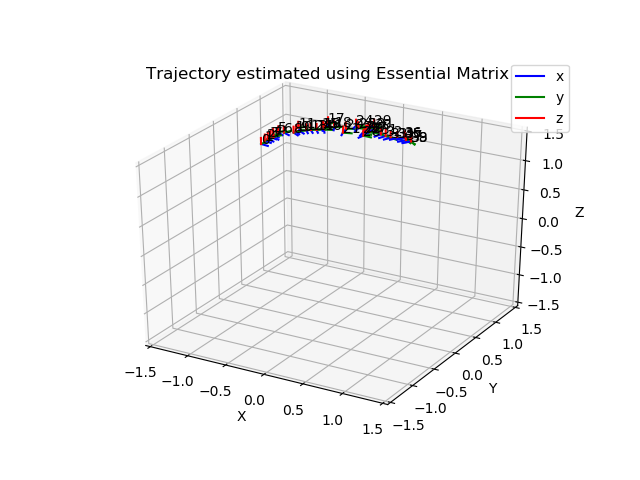
\includegraphics[width=80mm]{../2018-UAV-Registration/quad/basic-reg-saves/rtrj_rgb.png}
  \caption{Estimated trajectory for Essential Matrix method}
  \end{subfigure}%
  ~
  \begin{subfigure}[t]{0.5\textwidth}
  \centering
    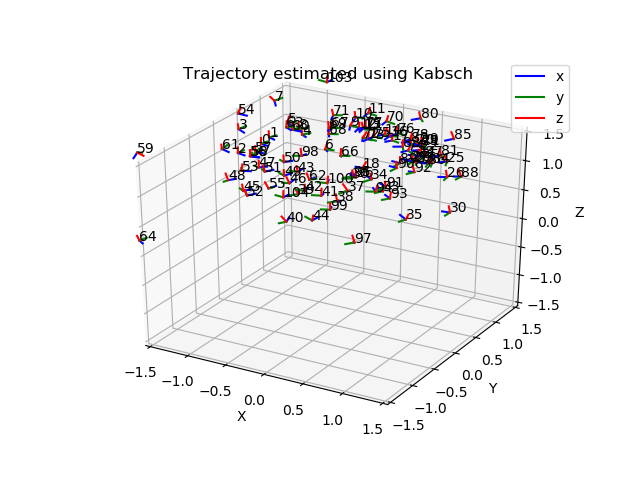
\includegraphics[width=80mm]{../2018-UAV-Registration/quad/basic-reg-saves/rtrj_d.png}
  \caption{Estimated trajectory for Kabsch method}
  \end{subfigure}
  \caption{Trajectory visualizations for first quad dataset}
  \label{f: quad1 trj}
\end{figure}

\begin{figure}[p]
  \centering
  \begin{subfigure}[t]{\textwidth}
  \centering
  \includegraphics[width=140mm]{../2018-UAV-Registration/quad/PCs/1533792217.77_PQ.png}
  \caption{Point clouds used for one frame of Kabsch}
  \end{subfigure}
  \\
  \begin{subfigure}[t]{0.5\textwidth}
  \centering
  \includegraphics[width=60mm]{../2018-UAV-Registration/quad/PCs/1533792217.77_PQ-aligned.png}
  \caption{Point clouds used for one frame of Kabsch, first point cloud P aligned with second point cloud Q using found rotation and translation}
  \end{subfigure}%
  ~
    \begin{subfigure}[t]{0.5\textwidth}
  \centering
  \includegraphics[width=60mm]{../2018-UAV-Registration/quad/PCs/1533792217.77_PQ-aligned-no.png}
  \caption{Point clouds used for one frame of Kabsch, first point cloud P aligned with second point cloud Q using found rotation with no translation}
  \end{subfigure}
  \caption{Kabsch point clouds for quadcopter. Currently using scaling factor = 1 which is too big.}
  \label{f: Kabsch quad good}
\end{figure}

\begin{figure}[p]
  \centering
  \begin{subfigure}[t]{\textwidth}
  \centering
  \includegraphics[width=140mm]{../2018-UAV-Registration/quad/PCs/1533792221.1_PQ.png}
  \caption{Point clouds used for one frame of Kabsch}
  \end{subfigure}
  \\
  \begin{subfigure}[t]{0.5\textwidth}
  \centering
  \includegraphics[width=60mm]{../2018-UAV-Registration/quad/PCs/1533792221.1_PQ-aligned.png}
  \caption{Point clouds used for one frame of Kabsch, first point cloud P aligned with second point cloud Q using found rotation and translation}
  \end{subfigure}%
  ~
    \begin{subfigure}[t]{0.5\textwidth}
  \centering
  \includegraphics[width=60mm]{../2018-UAV-Registration/quad/PCs/1533792221.1_PQ-aligned-no.png}
  \caption{Point clouds used for one frame of Kabsch, first point cloud P aligned with second point cloud Q using found rotation with no translation}
  \end{subfigure}
  \caption{Kabsch point clouds for quadcopter. Currently using scaling factor = 1 which is too big.}
  \label{f: Kabsch quad bad}
\end{figure}



\bibliographystyle{abbrvnat}
\bibliography{../Report/ENGN4217}

\end{document}